%%%%%%%%%%%%%%%%%%%%%%%%%%%%%%%%%%%%%%%%%%%%%%%%%%%%%%%%%%%%%%%%%%%%%%%%%%%%
\chapter{Large Language Models for Task-Oriented Dialogue}
\label{07:chap:lms}
%%%%%%%%%%%%%%%%%%%%%%%%%%%%%%%%%%%%%%%%%%%%%%%%%%%%%%%%%%%%%%%%%%%%%%%%%%%%

\label{07:sec:intro}
Large Language Models (LLMs) have transformed the NLP field,
showing outstanding performance across many NLP benchmarks such as Winograd Challenge \cite{levesque2012winograd} or GLUE \cite{wang2018glue}.
Recently, instruction finetuning of LLMs proved to be able to align the model outputs with human preferences \cite{ouyang2022training,supernaturalinstructions} and improved the LLMs' communication capabilities substantially.
State-of-the-art LLMs are not only good at understanding user needs but also capable of providing relevant answers.
%and even program code snippets.
Consequently, we see many chatbot applications both inside and outside academia (ChatGPT\footnote{\url{https://openai.com/blog/chatgpt}}, Claude\footnote{\url{https://www.anthropic.com/index/introducing-claude}}or BARD\footnote{\url{https://blog.google/technology/ai/bard-google-ai-search-updates/}}) which build upon the raw power of instruction-finetuned LLMs.

\section{Motivation}
Given the millions of daily interactions with these chatbots, it appears that the models are able to handle users' needs to their satisfaction, at least to some extent.
However, these chatbots are tuned using unstructured open-domain conversations.
We aim to evaluate these systems
for more specific applications, where the system has to follow a predetermined structure and handle external sources of information, such as APIs or databases.
We raise the question to what extent LLMs are capable of handling these applications off-the-shelf, i.e.\ without finetuning.
This approach, also frequently referred to as \emph{in-context learning} is a common way hoe to work with LLMs and offers competitive performance.
We  choose to evaluate LLM performance in the task-oriented dialogue (TOD) setting,
as it requires precise information handling for communicating with external APIs.
Moreover, TOD systems output in-domain information which has predetermined structure and lends itself well to evaluation, thanks to pre-existing annotated data sets.
We avoid finetuning techniques and focus on zero-shot or few-shot settings using in-context learning, as this approach has lower hardware requirements and barrier of entry and better flexibility or even performance in certain tasks \cite{su2022selective}.
It is important to note, that we cannot exclude a possibility that some of the models were exposed to our selected datasets during training.
However, we find it important to evaluate this setting as the real world use cases might largely rely on this approach.

In this chapter, we introduce an LLM-based TOD conversation pipeline and evaluate its performance with respect to commonly used task-oriented metrics such as Joint Goal Accuracy, Slot F1, and Dialogue Success \cite{rastogi_multi-task_2018,budzianowski_multiwoz_2018}.
Our pipeline resembles other approaches based on LMs \cite{peng-etal-2021-soloist,yang2021ubar}, using state tracking and response generation as two main, separate steps, while keeping the role of a dialogue policy implicit.
However, instead of finetuning LMs, it intentionally relies almost exclusively on the usage of pretrained LLMs as-is, so we can test their out-of-the-box capabilities.
The dialogue context and domain description are introduced to the model only by including them in the input prompt.
In the zero-shot setting, the model receives a domain description only; in the few-shot setting, it additionally uses a few retrieved examples (see Section~\ref{07:sec:method} for details).

In our experiments, we find that LLMs are not very good at state tracking and their performance falls behind state-of-the-art, task-specific trackers.
However, if provided with correct belief states, some of them yield interesting response generation performance, comparable to earlier finetuned state-of-the-art models.
Moreover, in our human evaluation experiments we show that LLMs are generally good with human interactions and their performance cannot be assesed only on the basis of automatic evaluations.

\section{Method}
\label{07:sec:method}
\begin{figure}[t]
    \centering
    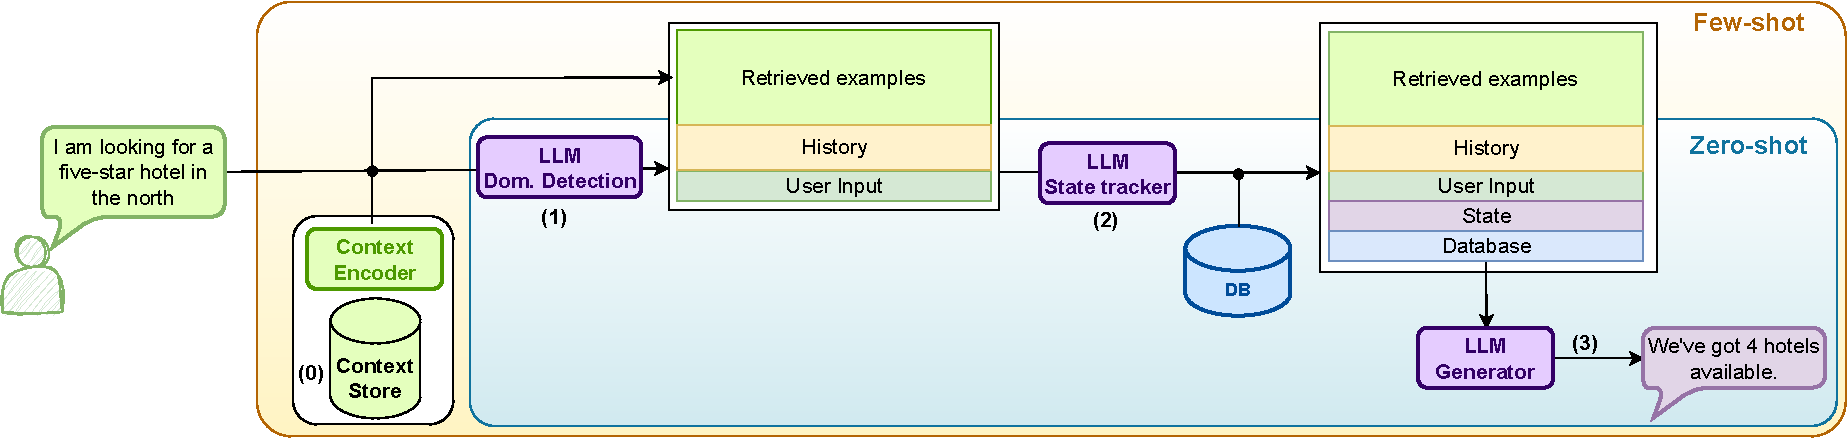
\includegraphics[width=\textwidth]{images/llm-chatbot-v3.pdf}
    \caption{A detailed description of our proposed pipeline. (0) As a preprocessing step, we encode a subset of the training set that will be used to retrieve few-shot examples.
    Given the user input, we: (1) Detect the domain, retrieve relevant examples (in the few-shot setting) and construct an initial prompt. (2) Infer the belief state using LLM. Based on that, we retrieve database information and construct another prompt that includes both the state and database results. (3) We ask the LLM to provide a final response.}
    \label{07:fig:overview_low_level}
\end{figure}
An overall description of the proposed pipeline is shown in Figure~\ref{07:fig:overview_low_level}.
The system consists of a pretrained LLM and an (optional) context store in a vector database.
We follow the 
Three LLM calls are performed in each dialogue turn, with specific prompts (see Section~\ref{sec:prompts}).
First, the LLM performs domain detection and state tracking (Section~\ref{07:sec:state-tracking}). The updated belief state informs a database query, whose results are used in the subsequent LLM-based response generation step (Section~\ref{07:sec:response-generation}).
In the few-shot setting, the context store is used to store a limited number of examples from the training set, which are retrieved based on similarity with the conversation context and included in LLM prompts (see Section~\ref{07:sec:context-store}).

%Retrieved examples are used to create a prompt for the LLM.
%The prompt also includes dialogue history, current utterance and potentially current belief state and database results.
%More technical details are included in Section \ref{sec:experiments}.


\subsection{Prompt construction}
\label{07:sec:prompts}
We aim to compare the raw capabilities of the selected LLMs, therefore we do not focus on prompt engineering techniques and choose universal prompts used for all LLMs in this work.
We choose simple, plain language statements as prompts, with no specific vocabulary, based only on a few preliminary tests.
We define a single \textbf{domain detection prompt} (Table~\ref{07_tab:domain}) for all examples, plus a pair of prompts for each domain in the given dataset: a \textbf{state tracking prompt} (Table~\ref{07_tab:zero-shot-state}) and a \textbf{response prompt} (Table~\ref{07_tab:zero-shot-response}).

The domain detection prompt includes a task description and two static examples of domain detection.
In addition to general instructions, each state tracking prompt contains a domain description, a list of relevant slots, the dialogue history, and the current user utterance.
The response prompts do not contain the per-domain slot list, but they include the current belief state and database results instead.
In the few-shot setting, each tracking and response prompt additionally contains positive and negative examples retrieved from the context store (see Section~\ref{07:sec:context-store}).

\begin{table}[H]
    \centering\small
    \begin{tabular}{rl}
      \toprule
      \textbf{Prompt} & \texttt{{\color{cyan!80!yellow!80!black!100 } Determine which domain is considered in the following}}\\
      & \texttt{{\color{cyan!80!yellow!80!black!100 }dialogue situation. }}\\
      & \texttt{ {\color{green!100!yellow!70!black!100 } Choose exactly one domain from this list:}}\\
      & \texttt{ {\color{green!100!yellow!70!black!100 }restaurant, hotel, attraction, taxi, train }} \\
      & \texttt{ {\color{cyan!80!yellow!80!black!100 } Answer with only one word, the selected domain from the list. }}\\
      & \texttt{ {\color{cyan!80!yellow!80!black!100 }You have to always select the most probable domain.}} \\
& \texttt{{\color{red!50!yellow!90!black!100!}  ------- Example 1: -------- }} \\
& \texttt{{\color{red!50!yellow!90!black!100!} Customer: I need a cheap place to eat}} \\
&\texttt{ {\color{red!50!yellow!90!black!100!} Assistant: We have several not expensive places available. }} \\
& \texttt{ {\color{red!50!yellow!90!black!100!}What food are you interested in?}} \\
& \texttt{{\color{red!50!yellow!90!black!100!} Customer: Chinese food.}} \\
& \texttt{{\color{red!50!yellow!90!black!100!}Domain: restaurant}} \\
& \texttt{{\color{red!50!yellow!90!black!100!} ------ Example 2: -------- } }\\
& \texttt{{\color{red!50!yellow!90!black!100!} Customer: What is the address?} } \\
&\texttt{{\color{red!50!yellow!90!black!100!} Assistant: It's 123 Northfolk Road. }} \\
& \texttt{ {\color{red!50!yellow!90!black!100!} Customer: That's all. I also need a train from London. }} \\
&  \texttt{{\color{red!50!yellow!90!black!100!} Domain: train }}\\
& \texttt{{\color{red!50!yellow!90!black!100!} ----------- }} \\
& \texttt{{\color{cyan!80!yellow!80!black!100 } Now complete the following example:}} \\
& \texttt{{\color{orange!50!yellow!90!black!100!} Customer: I am looking for a cheap place to stay. }}\\
& \texttt{Domain:} \\
      \midrule
      \textbf{Output:} & \texttt{hotel} \\
      \bottomrule
  \end{tabular}
    \caption{A prompt used for domain detection for MultiWOZ.
  It contains {\color{cyan!80!yellow!80!black!100} task definition},  {\color{green!100!yellow!70!black!100!}domains description}, {\color{red!50!yellow!90!black!100!} static examples} and {\color{orange!50!yellow!90!black!100!} user utterance}.}
  \label{07_tab:domain}
\end{table}

\begin{table}[H]
    \centering\small
    \begin{tabular}{rl}
      \toprule
      \textbf{Prompt} & \texttt{{\color{cyan!80!yellow!80!black!100 }Definition: Capture entity values from last utterance}}\\
      & \texttt{{\color{cyan!80!yellow!80!black!100 }of the conversation according to examples.}} \\
    & \texttt{{\color{cyan!80!yellow!80!black!100 } Capture pair "entity:value" separated by colon and no spaces}}\\ 
    & \texttt{{\color{cyan!80!yellow!80!black!100 }in between. Separate entity:value pairs by hyphens.}} \\
      & \texttt{{\color{cyan!80!yellow!80!black!100!} If not specified, leave the value empty.}}\\ 
      & \texttt{{\color{cyan!80!yellow!80!black!100!} Values that should be captured are: }} \\
      & \texttt{{\color{green!100!yellow!70!black!100!} - "pricerange": the price of the hotel} }\\
      & \texttt{{\color{green!100!yellow!70!black!100!} - "area" that specifies the area where the hotel is located}} \\
      & \texttt{{\color{green!100!yellow!70!black!100!}
      (north/east/west/south/centre)}} \\
      & \texttt{{\color{green!100!yellow!70!black!100!} - "internet" that specifies if the hotel has internet (yes/no)}} \\
      & \texttt{{\color{green!100!yellow!70!black!100!} - "parking" that specifies if the hotel has parking (yes/no)}} \\
      & \texttt{{\color{green!100!yellow!70!black!100!}- "stars" that specifies the quality of the hotel (1/2/3/4/5)}} \\
      & \texttt{{\color{green!100!yellow!70!black!100!} - "type" that specifies the type of the hotel}}\\
      & \texttt{{\color{green!100!yellow!70!black!100!}(hotel/bed and breakfast/guest house)}} \\
      & \texttt{{\color{red!100!yellow!70!black!100!}[history] }} \\
      &  \texttt{{\color{orange!50!yellow!90!black!100!}Customer: "I want a cheap place to stay." }}\\
      \midrule
      \textbf{Output:} & \texttt{pricerange:"cheap"}\\
      \bottomrule
  \end{tabular}
  \caption{A zero-shot version of the prompt used for state update prediction for MultiWOZ 2.2.
  It contains {\color{cyan!80!yellow!80!black!100} task definition},  {\color{green!100!yellow!70!black!100!}domain description}, {\color{red!100!yellow!70!black!100!} dialogue history} and {\color{orange!50!yellow!90!black!100!} user utterance}. }
  \label{07_tab:zero-shot-state}
\end{table}

\begin{table}[H]
    \centering\small
    \begin{tabular}{rl}
      \toprule
      \textbf{Prompt} & \texttt{{\color{cyan!80!yellow!80!black!100 }Definition: You are an assistant that helps people}} \\
      & \texttt{{\color{cyan!80!yellow!80!black!100} to book a hotel.}} \\
& \texttt{{\color{green!100!yellow!70!black!100 }The user can ask for a hotel by name, area, parking, }}\\
& \texttt{{\color{green!100!yellow!70!black!100 }internet availability, or price.}} \\
& \texttt{{\color{green!100!yellow!70!black!100 } There is also a number of hotel in the database currently }} \\
& \texttt{{\color{green!100!yellow!70!black!100 }corresponding to the user's request. }}\\
& \texttt{{\color{green!100!yellow!70!black!100 } If you find a hotel, provide [hotel\_name], [hotel\_address], }} \\
& \texttt{{\color{green!100!yellow!70!black!100 }[hotel\_phone] or [hotel\_postcode]}} \\
& \texttt{{\color{green!100!yellow!70!black!100 }Do not provide real entities in the response! Just provide}}\\
& \texttt{{\color{green!100!yellow!70!black!100 } entity name in brackets, like [name] or [address].} }\\
& \texttt{{\color{cyan!80!yellow!80!black!100 } If booking, provide [reference] in the answer. }} \\
& \texttt{{\color{red!100!yellow!70!black!100!}[history] }} \\
& \texttt{{\color{orange!50!yellow!90!black!100!}Customer: "I want a cheap place to stay." }}\\
& \texttt{{\color{magenta!100!yellow!70!black!100!}State: hotel \{ pricerange: "cheap"\} }} \\
& \texttt{{\color{magenta!100!yellow!70!black!100!} Database: hotels: 23 }}\\
      \midrule
      \textbf{Output:} & \texttt{We have 23 such hotels available,} \\
      & \texttt{do you have a location preference?} \\
      \bottomrule
  \end{tabular}
  \caption{A zero-shot version of the prompt used for response prediction for MultiWOZ 2.2.
  It contains {\color{cyan!80!yellow!80!black!100} task definition},  {\color{green!100!yellow!70!black!100!}domain description}, {\color{red!100!yellow!70!black!100!} dialogue history}, {\color{orange!50!yellow!90!black!100!} user utterance} and {\color{magenta!100!yellow!70!black!100!} belief state with db results}.}
  \label{07_tab:zero-shot-response}
\end{table}
\subsection{Domain Detection and State Tracking}
\label{07:sec:state-tracking}

We prompt the LM twice at each turn during state tracking: first, to detect the active domain, then to output slot values that changed or appeared in the current turn. We then use the outputs to update the accumulated global belief state.

The two prompting steps are used since 
we need the models to operate in a multi-domain setting, i.e., handle conversations spanning multiple domains.
Therefore, we need to be able to detect the current active domain.
%Therefore, we intentionally retrieve more examples than needed from the context store and detect the domain by majority voting among the retrieved entries.
We achieve this by first prompting the LLM with a domain detection prompt (using a single prompt for all examples).
%This prompt is static, i.e., it remains the same for each example.

Once we obtain the active domain prediction, we can include manually designed domain descriptions in a second prompt that handles belief state prediction.
An example of a prompt used for state tracking is provided in Table~\ref{07_tab:zero-shot-state}.
For the few-shot variants, %the retrieved context provides additional information.
%, 
we retrieve few-shot examples from the context store, limited to the active domain.\footnote{For this purpose, each conversation snippet contained in the context store comes from a single-domain conversation.}

Our preliminary experiments showed that LLMs struggle to output all active slot values at every turn consistently.
Therefore, we model only state updates, following the MinTL approach \cite{lin-etal-2020-mintl}.
Here, the model only generates the slot-value pairs that have changed in the current turn.
The global belief state is then accumulated using these turn-level updates.
To obtain machine-readable outputs useful for database queries or API calls,
we specify in the prompt that the model should provide JSON outputs, and any provided few-shot examples are formatted accordingly. 
The current belief state is used to query the database for entries matching all user-specified slots in the active domain. Given the belief state and database results, the response generation is straightforward.
The prompt for the LLM includes dialogue history, user utterance, belief state and database results (and retrieved examples in the few-shot setting) and requests the model to provide a fitting system response.
We generate delexicalized responses \cite{wen-etal-2015-stochastic}, i.e., we replace slot values by placeholders, following prior work in end-to-end TOD modeling.
%\OD{a funguje to tak doopravdy? nedela nam to problem s evaluaci, ze model negeneruje placeholdery, ale ty skutecne hodnoty?}
In addition to simplifying the task for the model, delexicalized outputs allow us to evaluate the success rate and compare to previous works.
The prompt specifies that the model should provide entity values as delexicalized placeholders and any few-shot examples are constructed accordingly.

\subsection{Context Storage}
\label{07:sec:context-store}
It has been shown that enriching prompts with specific examples (i.e. \emph{few-shot prompting}) boosts LM performance \cite{madotto2020language,brown2020language}.
To apply this knowledge efficiently in our pipeline, we introduce a storage that contains encoded dialogue contexts.
This context storage is optional and is only required for the few-shot prompting variant.
We use dialogue context taken from a fixed-length history window as the key to be encoded in the vector database.
Once the relevant examples are retrieved, we include them in the prompt to guide the model better.
Some of the LLMs rely on negative (counter-) examples as well \cite{supernaturalinstructions}, hence we take some of the retrieved belief state examples, corrupt them by replacing some of the correct slot values with random values, and present them as negative in the prompt.

\section{Experimental Setup}
\label{07:sec:experiments}

To obtain a broad overview of the current LLMs' capabilities, we compare several models, spanning different numbers of trainable parameters and different training methods. 
We also experiment with four variants of the base setup, using either zero-shot or few-shot operations and using either predicted or oracle belief states.

\subsection{Tested Models}
We chose the following five instruction-finetuned models for our experiments, spanning different sizes (within the limitations of hardware available to us) and using freely available models as well as the paid ChatGPT API.
We indicate the specific model variant (i.e., model size, given by the number of parameters) directly in the model name.
\label{07:sec:par:models}
\begin{itemize}
    \item \textbf{Tk-Instruct-11B} \cite{supernaturalinstructions} is based on the T5 encoder-decoder architecture \cite{2020t5}. It was tuned on a dataset of over 5M task instances with instructions.
    \item \textbf{ChatGPT} is a product introduced by OpenAI.\footnote{\url{https://openai.com/blog/chatgpt}} Although the exact training process and architectures were not published, it most probably uses a similar architecture and finetuning techniques as InstructGPT \cite{ouyang2022training}, with additional human feedback.
    \item \textbf{Alpaca-LoRA-7B} is a version of the LLaMa model \cite{touvron2023llama} using the LoRA method \cite{hu2021lora} for finetuning on Stanford Alpaca project data \cite{alpaca}. LoRa keeps the base model parameters frozen, but adds additional smaller weight matrices to the model to transform its outputs.
    \item \textbf{GPT-NeoXT-Chat-Base-20B} is based on the GPT-NeoX open-source language model \cite{black2022gpt} and finetuned with over 40M dialogue-style instructions.
    \item \textbf{OPT-IML-30B} \cite{iyer2022opt} is based on the Transformer decoder OPT model \cite{zhang2022opt} and trained with a custom set of instructions, including the finetuning set from Tk-Instruct.
\end{itemize}

\subsection{Evaluated variants}
We test four variants of our setup for each pair of model and dataset.
Specifically, we use zero-shot (without examples) or few-shot (including examples) prompts (\emph{-zs-} vs. \emph{-fs-}) and either generated or oracle belief states (\emph{-gbs} vs. \emph{-obs}).
For retrieval in the few-shot setting, we store just 10 examples per domain in the context store by default. We experiment with increasing this number in Section~\ref{07:sec:dialogue-performance}.
Using oracle belief state allows us to focus on evaluating the LLM's ability to guide the dialogue.

\subsection{Experiment Details}
\label{subsec:exp-details}
Due to the expensiveness of the LLM runs,\footnote{Hardware intensity for the freely available models and actual cost for ChatGPT.} we did not perform a grid search, but used a limited set of preliminary experiments to determine hyperparameters.
Based on this, we used the context of two preceding  utterances (user + system) as the context store keys (cf.~Section~\ref{sec:context-store}).
We retrieve two examples for few-shot prompts and make one corrupted variant from each of them for negative examples.
To corrupt an example, we switch some of the slot values randomly, similarly to \citet{kulhanek-etal-2021-augpt}.
In the context store, we encode few-shot examples using the multilingual embedding model provided by \citet{reimers-2020-multilingual-sentence-bert}\footnote{\url{https://huggingface.co/sentence-transformers/all-mpnet-base-v2}} and store them in the FAISS database \cite{johnson2019billion}.
To perform the LLM calls, we use the Huggingface library\footnote{\url{https://huggingface.co}} and the OpenAI API.\footnote{\url{https://platform.openai.com}}

\subsection{Evaluation Measures}

We evaluate the system outputs on multiple levels, both using automatic metrics and human evaluation. Results are given in Sections~\ref{07:sec:results} and~\ref{07:sec:analysis}, respectively.
For details about the used metrics, please see Section~\ref{02:sec:eval_metrics}.
\subsubsection*{Automatic Metrics}
In automatic evaluation, we first follow the LLM calls being made and evaluate domain detection, state tracking as well as response generation. We also evaluate the overall dialogue-level performance.
For \emph{domain detection}, we simply compute \textbf{detection accuracy}.
For \emph{state tracking}, we compute \textbf{micro-F1} score and \textbf{Joint Goal Accuracy} (JGA).
To evaluate \emph{response generation}, we follow related works and use \textbf{BLEU score}.
The main \emph{overall measure} for evaluating a task-oriented dialogue is the dialogue \textbf{success rate} \cite{deriu_survey_2021}.

\subsubsection*{Human Evaluation}
For human evaluation, we perform a small-scale in-house interaction study on MultiWOZ.
Since the MultiWOZ goal often involves tasks in multiple domains, we ask annotators to evaluate each domain in the dialogue distinctly.
At the end of each dialogue, the annotators are asked to answer these questions:
\begin{enumerate}
    \item \emph{How many of the subdialogues/domains were handled successfully?} (corresponding to dialogue success)
    \item \emph{How many clarifications or corrections were needed?}
    \item \emph{Was all the provided information captured correctly?} (corresponding to JGA)
\end{enumerate}

\begin{figure}[h]
    \centering
    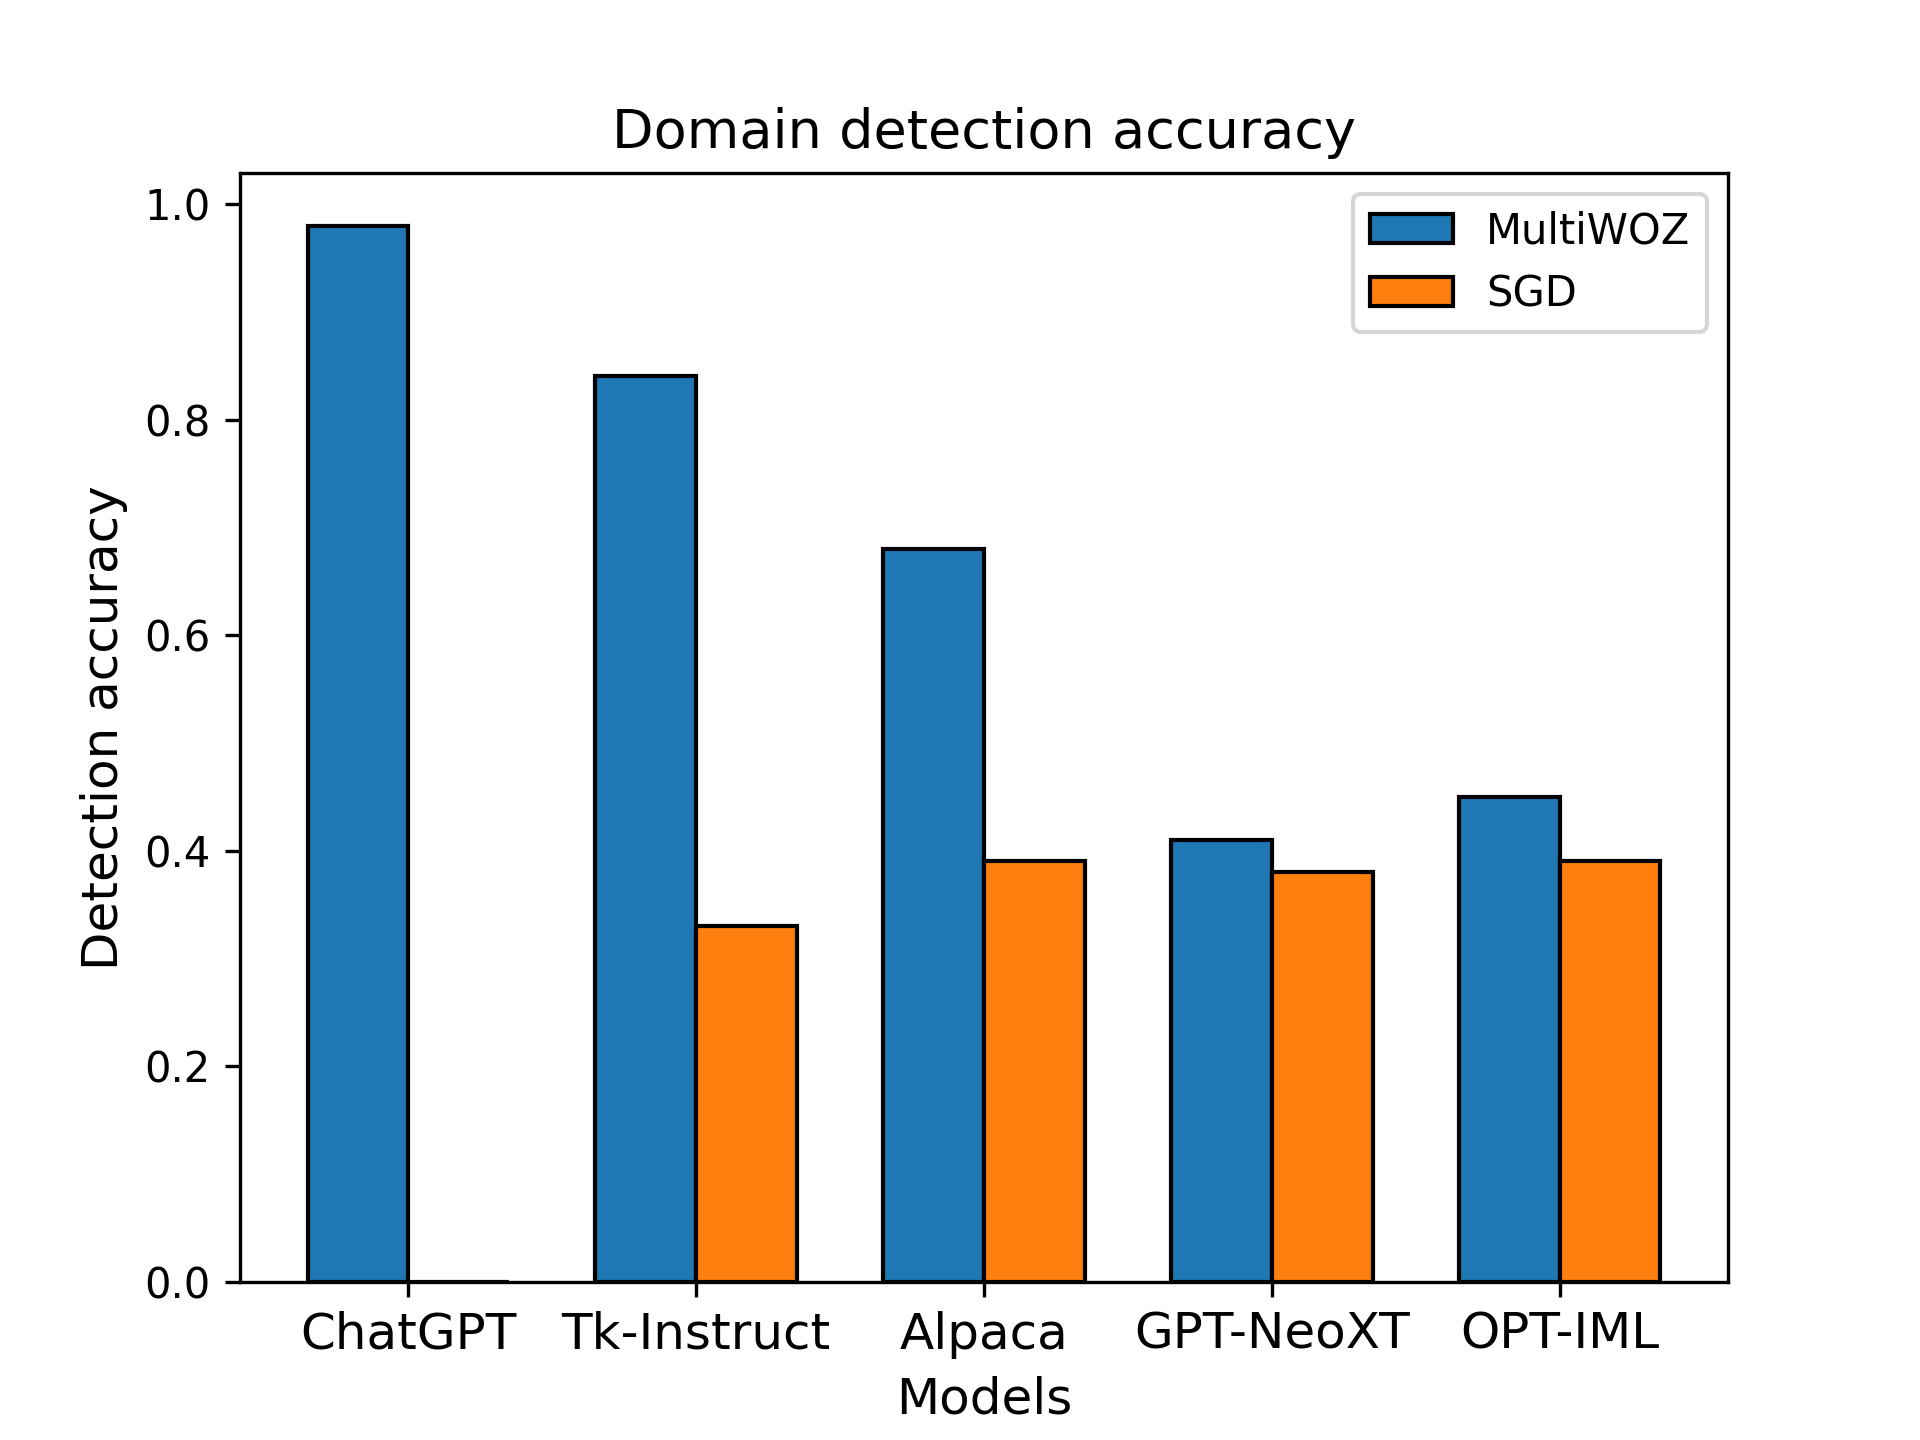
\includegraphics[width=0.49\textwidth]{images/domain-detections.png}
    \caption{Domain detection accuracy with respect to different models for MultiWOZ 2.2 and SGD data wchich consist of 7 and 18 domains, respectively.}
    \label{07:fig:domains}
\end{figure}


\section{Automatic Metrics Results}
\label{sec:results}

\subsection{Domain detection}
\label{subsec:domain}
We report the domain detection accuracy on MultiWOZ and SGD
in Figure~\ref{fig:domains}.
We observe that the domain detection accuracy varies quite a lot for various models and presumably influences the quality of the retrieved few-shot examples and appropriateness of the subsequent prompts.
However, it is important to note that domain detection is turn-based, and arguably there are situations (e.g. providing an address, saying goodbye etc.) that are always handled in the same fashion, even though they formally belong to different domains.
Therefore, not all the retrieved examples from misclassified domains necessarily contain unrelated contexts.
To explore this, we measure the performance of all models in case an oracle domain is given to them (Figure \ref{fig:oracle_domains}).
Interestingly, using the oracle domain did not improve performance, it even worsened in some cases.
This suggests that the model-predicted domain is generally good enough, and additionally providing the domain information does not contribute to the final system performance.
The negative influence on performance might be caused by forcing the system to filter out relevant examples.
We observe that in multiple cases, the conversations snippets are domain-independent so the retrieval might perform better even with a wrongly selected domain.
Forcing the ground truth domain examples in these cases can be potentially harmful.

%%%%%%%%%%%%%%%%%%%%%%%%%
% FIG 4 - oracle domain
%%%%%%%%%%%%%%%%%%%%%%%%%
\begin{figure}[h]
    \centering
    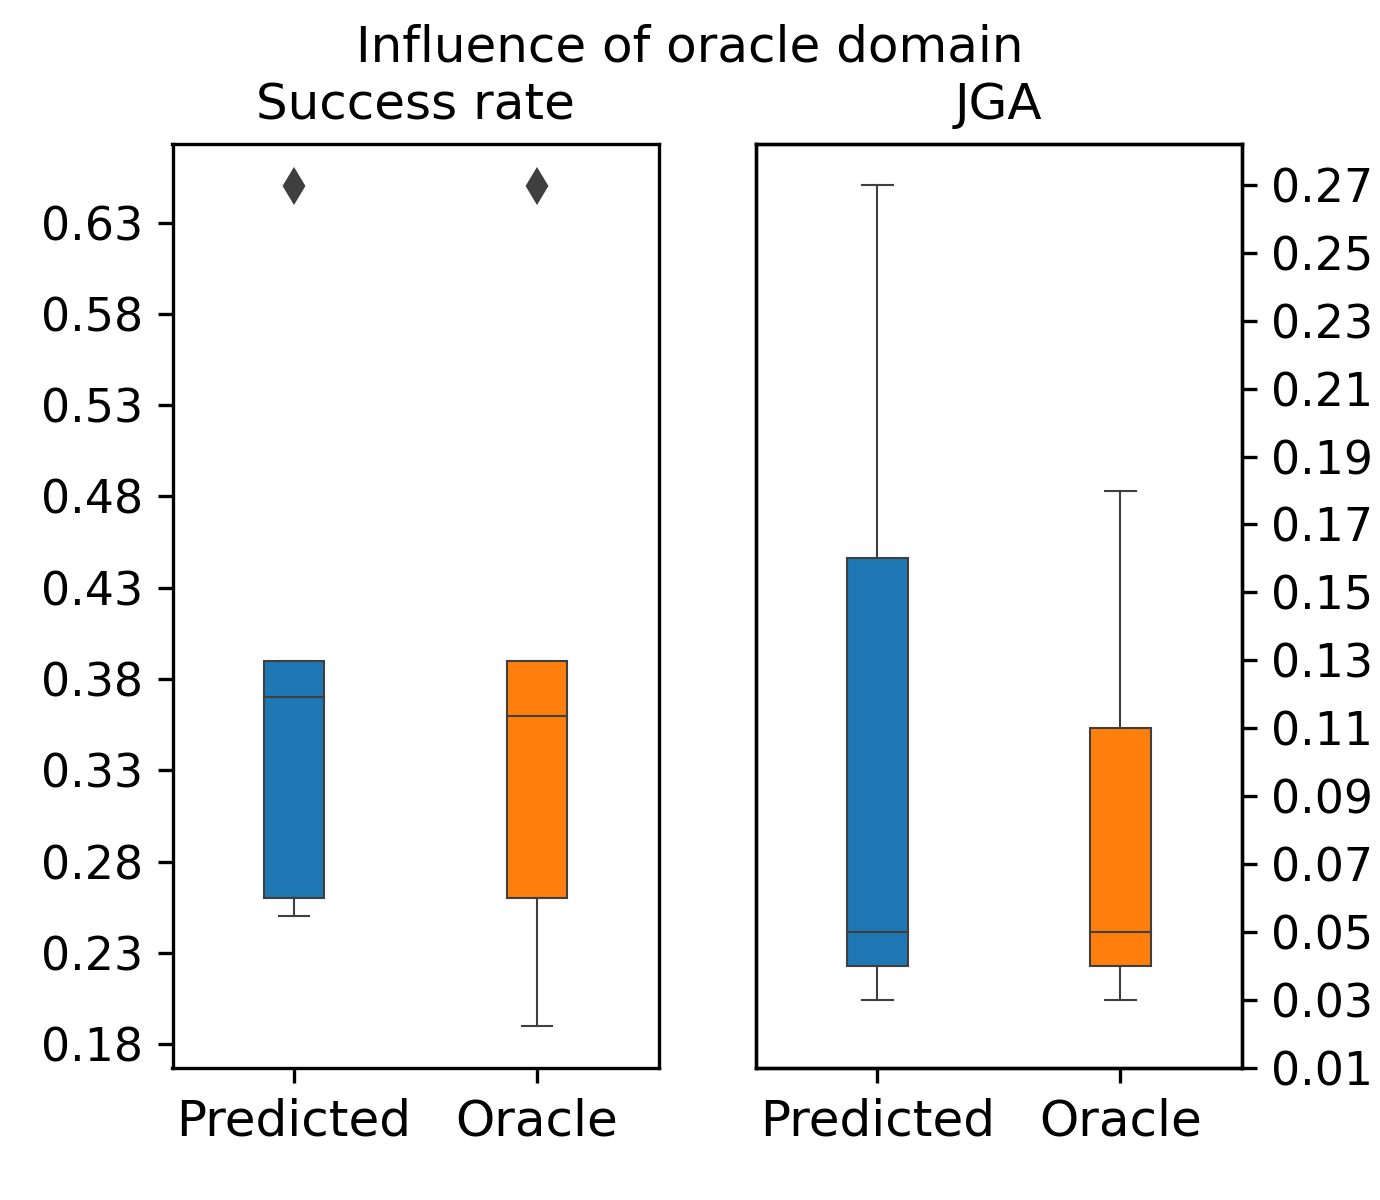
\includegraphics[width=0.49\textwidth]{images/oracle_domains.png}
    \caption{The influence of using oracle domain to retrieve examples. Interestingly, the oracle domain does not improve the performance, suggesting that the model-based detection is good enough for retrieval.}
    \label{fig:oracle_domains}
\end{figure}

\begin{table}[h]
    \centering\small
    \begin{tabular}{l|c|c|ccc>{\hspace{-2mm}}c}
      \toprule
      model & few & oracle & \multicolumn{4}{c}{\textbf{MultiWOZ 2.2}} \\
      & shot & BS & BLEU & JGA & Slot-F1 & Success \\
      \midrule
      % Baselines
      Supervised SotA & \textcolor{red}{\xmark} & \textcolor{red}{\xmark} & 19.90$^\clubsuit$ & 0.60$^\diamondsuit$ & -- & 0.82$^\heartsuit$ \\
      % few-shot SotA & \textcolor{green}{\cmark} & \textcolor{red}{\xmark} & --& -- & -- & -- & BLEU & JGA & Slot-F1 & Success \\
      \midrule
      % ZS-GBS
      \rowcolor{tablegray}
      \emph{Alpaca-LoRA-7B-zs-gbs} & \textcolor{red}{\xmark} & \textcolor{red}{\xmark} & 1.61 & 0.06 & 0.07 & 0.04 \\
      \rowcolor{tablegray}
      \emph{Tk-Instruct-11B-zs-gbs} & \textcolor{red}{\xmark} & \textcolor{red}{\xmark} & 2.48 & 0.04 & 0.04 & 0.04 \\
      \rowcolor{tablegray}
      \emph{GPT-NeoXT-20B-zs-gbs} & \textcolor{red}{\xmark} & \textcolor{red}{\xmark} & 0.52 & 0.03 & 0.02 & 0.04 \\
      \rowcolor{tablegray}
      \emph{OPT-IML-30B-zs-gbs} & \textcolor{red}{\xmark} & \textcolor{red}{\xmark} & 0.56 & 0.02 & 0.04 & 0.03 \\
      \rowcolor{tablegray}
      \emph{ChatGPT-zs-gbs} & \textcolor{red}{\xmark} & \textcolor{red}{\xmark} & 4.17 & 0.13 & 0.40 & 0.31 \\ 

      % ZS-OBS
      \emph{Alpaca-LoRA-7B-zs-obs} & \textcolor{red}{\xmark} & \textcolor{green}{\cmark} & 1.73 & -- & -- & 0.08 \\
      \emph{Tk-Instruct-11B-zs-obs} & \textcolor{red}{\xmark} & \textcolor{green}{\cmark} & 2.66 & -- & -- & 0.18 \\
      \emph{GPT-NeoXT-20B-zs-obs} & \textcolor{red}{\xmark} & \textcolor{green}{\cmark} & 0.60 & -- & -- & 0.06 \\
      \emph{OPT-IML-30B-zs-obs} & \textcolor{red}{\xmark} & \textcolor{green}{\cmark} & 0.54 & -- & -- & 0.06 \\
      \emph{ChatGPT-zs-obs} & \textcolor{red}{\xmark} & \textcolor{green}{\cmark} & 3.76 & -- & -- & 0.47 \\ \midrule

      % FS- GBS
      \rowcolor{tablegray}
      \emph{Alpaca-LoRA-7B-fs-gbs} & \textcolor{green}{\cmark} & \textcolor{red}{\xmark} & 5.53 & 0.06 & 0.08 & 0.06\\
      \rowcolor{tablegray}
      \emph{Tk-Instruct-11B-fs-gbs} & \textcolor{green}{\cmark} & \textcolor{red}{\xmark} & 6.56 & 0.16 & 0.33 & 0.19 \\
      \rowcolor{tablegray}
      \emph{GPT-NeoXT-20B-fs-gbs} & \textcolor{green}{\cmark} & \textcolor{red}{\xmark} & 2.73 & 0.05 & 0.04 & 0.05 \\
      \rowcolor{tablegray}
      \emph{OPT-IML-30B-fs-gbs} & \textcolor{green}{\cmark} & \textcolor{red}{\xmark} & 4.40 & 0.03 & 0.03 & 0.04 \\
      \rowcolor{tablegray}
      \emph{ChatGPT-fs-gbs} & \textcolor{green}{\cmark} & \textcolor{red}{\xmark} & 6.77 & \textbf{0.27} & \textbf{0.51} & 0.44 \\

      % FS-OBS
      \emph{Alpaca-LoRA-7B-fs-obs} & \textcolor{green}{\cmark} & \textcolor{green}{\cmark} & 5.96 & -- & -- & 0.41 \\
      \emph{Tk-Instruct-11B-fs-obs} & \textcolor{green}{\cmark} & \textcolor{green}{\cmark} & \textbf{6.91} & -- & -- & 0.46 \\
      \emph{GPT-NeoXT-20B-fs-obs} & \textcolor{green}{\cmark} & \textcolor{green}{\cmark} & 2.92 & -- & -- & 0.28 \\
      \emph{OPT-IML-30B-fs-obs} & \textcolor{green}{\cmark} & \textcolor{green}{\cmark} & 5.40 & -- & -- & 0.28 \\
      \emph{ChatGPT-fs-obs} & \textcolor{green}{\cmark} & \textcolor{green}{\cmark} & 6.84 & -- & -- & \textbf{0.68} \\
     
    \bottomrule
  \end{tabular}
  \caption{
  Evaluation of the chosen LLMs with respect to widely used TOD measures on the MultiWOZ dataset. For each model, we provide multiple variants. We use either zero-shot or few-shot prompts (\emph{-zs-} vs. \emph{-fs-}) and either generated or oracle belief state (\emph{-gbs} vs. \emph{-obs}).
  The few-shot variants use 10 examples per domain in the context storage two of which are selected for the prompts.  We also provide supervised state-of-the-art results to put the numbers in context: $^\ast$\citet{zhu2022convlab3}, $^\dagger$\citet{feng-etal-2021-sequence}, $^\clubsuit$\citet{sun2022mars}, $^\diamondsuit$\citet{huangrobustness}, $^\heartsuit$\citet{feng2023fantastic}. }
  \label{tab:res_overall}
\end{table}


\subsection{Belief State Tracking}
\label{subsec:dst}
The belief state tracking results overview is given in Table \ref{tab:res_overall} (\emph{JGA} and \emph{Slot-F1}).
There is a huge gap between the supervised models' performance and the LLM results.
Also compared to \citet{hu-etal-2022-context}, who used few-shot in-context learning and reported JGA 43.13\% with a comparable dataset size, our instruction-tuned LLMs fall short.
However, the models we use are an order of magnitude smaller in general, and we also use fewer examples in the prompt.
We hypothesize that the performance could be further improved by careful model-specific prompt customization and perhaps task re-formulation; nevertheless, this is not the goal of this work.
We intentionally focus on the universal framing of the task since we want to explore the general ability of the models to follow instructions.

When comparing the results among the models, ChatGPT clearly outperforms the rest of the models by a large margin. 
Interestingly, the few-shot vs.\ zero-shot setting does not seem to influence the results much, except for the GPT-NeoXT model.

\subsection{Response Generation}
\begin{table}[h]
    \centering\small
    \begin{tabular}{l|c|c|ccc>{\hspace{-2mm}}c}
      \toprule
      model & few & oracle & \multicolumn{4}{c}{\textbf{Schema Guided Dialogues}} \\
      & shot & BS & BLEU & JGA & Slot-F1 & Success  \\
      \midrule
      % Baselines
      Supervised SotA & \textcolor{red}{\xmark} & \textcolor{red}{\xmark} & 29.90$^\ast$ & 0.30$^\dagger$ & 0.60$^\ast$ & --  \\
      % few-shot SotA & \textcolor{green}{\cmark} & \textcolor{red}{\xmark} & --& -- & -- & -- & BLEU & JGA & Slot-F1 & Success \\
      \midrule
      % ZS-GBS
      \rowcolor{tablegray}
      \emph{Alpaca-LoRA-7B-zs-gbs} & \textcolor{red}{\xmark} & \textcolor{red}{\xmark} & 2.79 & 0.02 & 0.01 & 0.11  \\
      \rowcolor{tablegray}
      \emph{Tk-Instruct-11B-zs-gbs} & \textcolor{red}{\xmark} & \textcolor{red}{\xmark} & 4.16 & 0.05 & 0.03 & 0.10  \\
      \rowcolor{tablegray}
      \emph{GPT-NeoXT-20B-zs-gbs} & \textcolor{red}{\xmark} & \textcolor{red}{\xmark} & 0.45 & 0.01 & 0.01 & 0.17 \\
      \rowcolor{tablegray}
      \emph{OPT-IML-30B-zs-gbs} & \textcolor{red}{\xmark} & \textcolor{red}{\xmark} & 1.63 & 0.01 & 0.01 & 0.17 \\
      \rowcolor{tablegray}
      % \emph{ChatGPT-zs-gbs} & \textcolor{red}{\xmark} & \textcolor{red}{\xmark} & -- & -- & -- & --  \\ 

      % ZS-OBS
      \emph{Alpaca-LoRA-7B-zs-obs} & \textcolor{red}{\xmark} & \textcolor{green}{\cmark} & 2.76 & -- & -- & 0.23  \\
      \emph{Tk-Instruct-11B-zs-obs} & \textcolor{red}{\xmark} & \textcolor{green}{\cmark} & 5.21 & -- & -- & 0.24  \\
      \emph{GPT-NeoXT-20B-zs-obs} & \textcolor{red}{\xmark} & \textcolor{green}{\cmark} & 0.83 & -- & -- & 0.22  \\
      \emph{OPT-IML-30B-zs-obs} & \textcolor{red}{\xmark} & \textcolor{green}{\cmark} & 1.94 & -- & -- & 0.22  \\
      % \emph{ChatGPT-zs-obs} & \textcolor{red}{\xmark} & \textcolor{green}{\cmark} & -- & -- & -- & --  \\ \midrule

      % FS- GBS
      \rowcolor{tablegray}
      \emph{Alpaca-LoRA-7B-fs-gbs} & \textcolor{green}{\cmark} & \textcolor{red}{\xmark} & 6.32 & 0.04 & 0.01 & 0.09 \\
      \rowcolor{tablegray}
      \emph{Tk-Instruct-11B-fs-gbs} & \textcolor{green}{\cmark} & \textcolor{red}{\xmark} & 6.66 & 0.06 & 0.05 & 0.10 \\
      \rowcolor{tablegray}
      \emph{GPT-NeoXT-20B-fs-gbs} & \textcolor{green}{\cmark} & \textcolor{red}{\xmark} & 1.62 & 0.04 & 0.02 & 0.09  \\
      \rowcolor{tablegray}
      \emph{OPT-IML-30B-fs-gbs} & \textcolor{green}{\cmark} & \textcolor{red}{\xmark} & 0.82 & \textbf{0.06} & \textbf{0.07} & 0.08  \\
      \rowcolor{tablegray}
      % \emph{ChatGPT-fs-gbs} & \textcolor{green}{\cmark} & \textcolor{red}{\xmark} & -- & -- & -- & --  \\

      % FS-OBS
      \emph{Alpaca-LoRA-7B-fs-obs} & \textcolor{green}{\cmark} & \textcolor{green}{\cmark} & 6.99 & -- & -- & \textbf{0.25} \\
      \emph{Tk-Instruct-11B-fs-obs} & \textcolor{green}{\cmark} & \textcolor{green}{\cmark} & \textbf{8.56} & -- & -- & \textbf{0.25} \\
      \emph{GPT-NeoXT-20B-fs-obs} & \textcolor{green}{\cmark} & \textcolor{green}{\cmark} & 1.97 & -- & -- & 0.24 \\
      \emph{OPT-IML-30B-fs-obs} & \textcolor{green}{\cmark} & \textcolor{green}{\cmark} & 0.56 & -- & -- & 0.22 \\
      % \emph{ChatGPT-fs-obs} & \textcolor{green}{\cmark} & \textcolor{green}{\cmark} & -- & -- & -- & -- \\

    \bottomrule
  \end{tabular}
  \caption{
  Evaluation of the chosen LLMs with respect to widely used TOD measures on the SGD dataset. For each model, we provide multiple variants. We use either zero-shot or few-shot prompts (\emph{-zs-} vs. \emph{-fs-}) and either generated or oracle belief state (\emph{-gbs} vs. \emph{-obs}).
  The few-shot variants use 10 examples per domain in the context storage, two of which are selected for the prompts.
  To reduce cost, we didn't  evaluate the paid ChatGPT model on SGD.
  We also provide supervised state-of-the-art results to put the numbers in context: $^\ast$\citet{zhu2022convlab3}, $^\dagger$\citet{feng-etal-2021-sequence}, $^\clubsuit$\citet{sun2022mars}, $^\diamondsuit$\citet{huangrobustness}, $^\heartsuit$\citet{feng2023fantastic}. }
  \label{tab:res_overall}
\end{table}


BLEU scores are low overall, far below the supervised state-of-the-art. Tk-Instruct and ChatGPT are the strongest here and perform roughly on par.

\subsection{Dialogue-level performance}
\label{sec:dialogue-performance}
\begin{figure}[t]
    \centering
    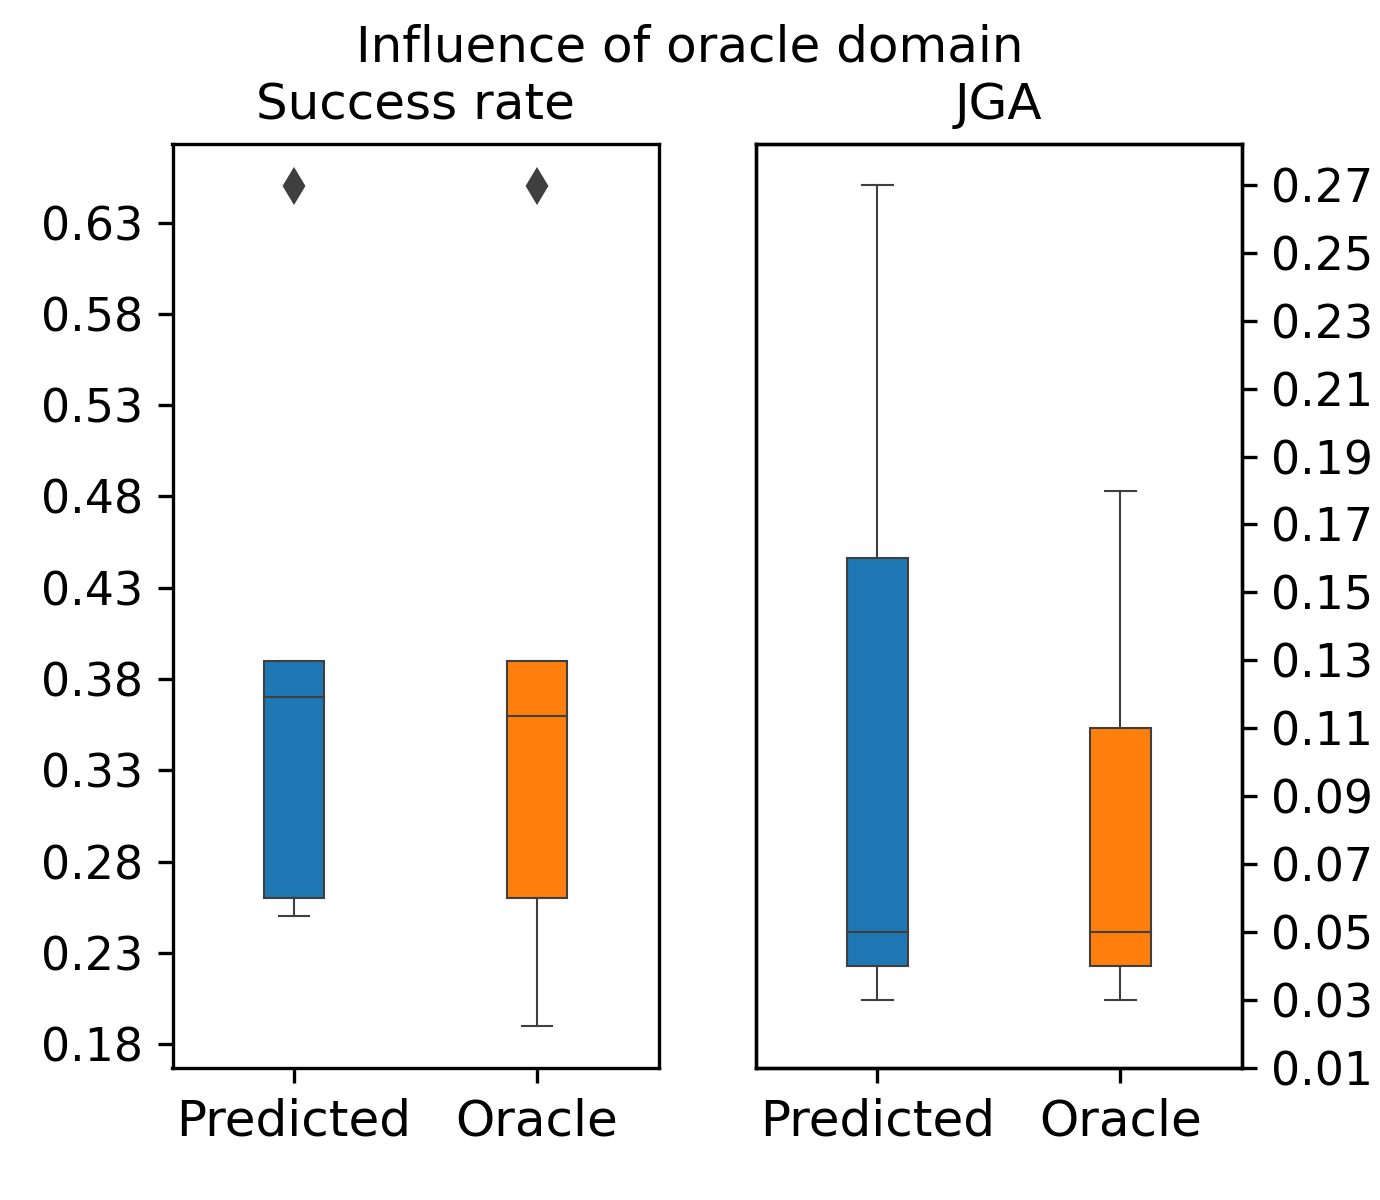
\includegraphics[width=0.49\textwidth]{images/oracle_domains.png}
    \caption{The influence of using oracle domain to retrieve examples. Interestingly, the oracle domain does not improve the performance, suggesting that the model-based detection is good enough for retrieval.}
    \label{07:fig:oracle_domains}
\end{figure}
%The ultimate measure to evaluate a task-oriented dialogue model is dialogue success.
Results for dialogue success are provided in Table~\ref{tab:res_overall}, and there is again a large gap between LLMs and supervised custom models' performance.
ChatGPT seems to outperform other models, similarly to state tracking (cf.~Section~\ref{subsec:dst}).
However, for some cases, especially in the zero-shot setting, the difference is not that obvious.
In most cases, adding the retrieved few-shot examples helps.
The contribution of retrieved examples is more obvious when we supply the oracle belief state, in which case it helps consistently for all the models.

We also explore the influence of context storage size on the dialogue success rate.
The results are given in Figure~\ref{fig:shots}.
It seems that the biggest improvement can be achieved by supplying just a few examples instead of zero-shot prompting, but increasing the size of the example pool for retrieval does not yield further performance gains.
\begin{figure}[h]
    \centering
    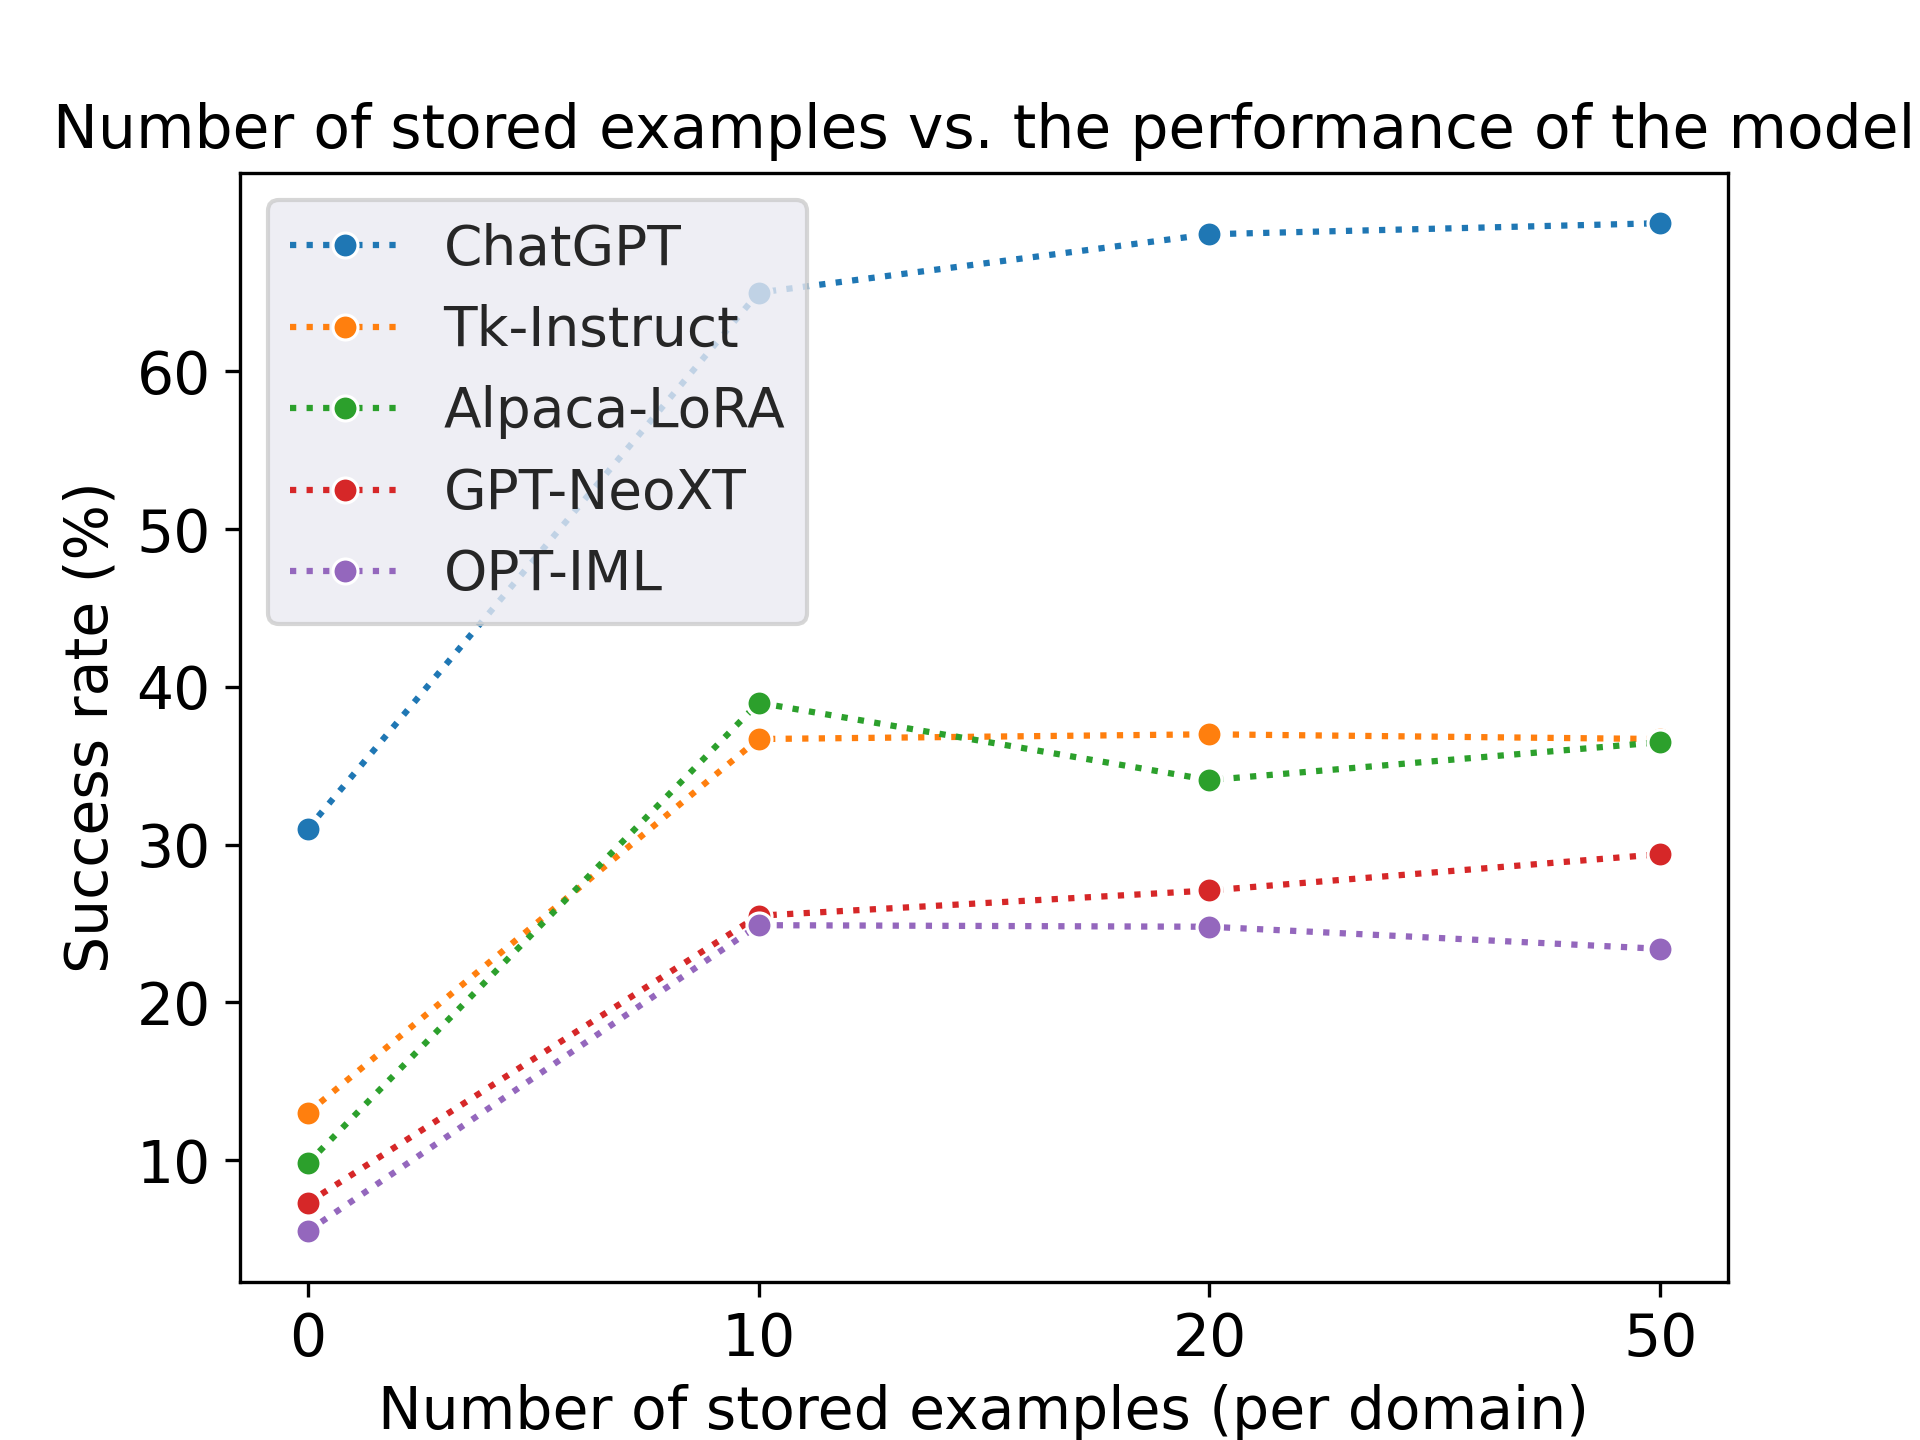
\includegraphics[width=0.49\textwidth]{images/shots.png}
    \caption{The influence of the number of examples per domain available for few-shot retrieval and performance of the model in terms of the dialogue success on MultiWOZ 2.2 data with oracle state supplied. Note that this does not represent the number of examples selected for the prompt, which is fixed to two.}
    \label{07:fig:shots}
\end{figure}

\section{Model Analysis}
\label{sec:analysis}

%It is important to understand the LLM's behavior not just quantitatively but more in-depth.
%Therefore we perform human evaluation and detailed error analysis to obtain more insights.

\subsection{Human Evaluation}

We employed 6 annotators with a background in linguistics and NLP and let them interact with the two strongest models in terms of automatic metrics: ChatGPT and Tk-Instruct.
The annotators were given randomly selected goals from the MultiWOZ 2.2 dataset and a minimal set of essential instructions on how to proceed.
We present the results in Table~\ref{tab:human}.
We can see that in a real interaction with a human user and allowing for clarification or correction, the models perform better compared to the rather strict automatic evaluation.
Furthermore, the models are often successful in multiple subdialogues, even if a part of the whole dialogue fails.
The experiment also confirms the superior performance of ChatGPT on both dialogue success and JGA.
Not surprisingly given the above results, conversations with ChatGPT also required fewer clarification turns than with Tk-Instruct.

\subsection{Error Analysis}

To understand the models' behavior better, we manually inspect a random sample of ca.~20 dialogues for each model, chosen from cases where the automatic success metric was not satisfied. 
In general, we can split most of the erroneous behaviors into two distinct groups, which we call \emph{prompt-recoverable} and \emph{inherent}.

\paragraph{Prompt-recoverable errors} can be likely fixed by specific prompt engineering with some effort.
These kind of errors happen with all of the tested models.
Examples of such errors are invalid structure of the generated dialogue state, copying slot values instead of using canonical values from the ontology, failure to delexicalize some of the values, etc.
Most of these errors can be also fixed in postprocessing -- for example, we can employ more robust parsers or fuzzy matching of slot values.

\paragraph{Inherent errors,} on the other hand, are likely not easily fixable by prompt modifications.
They are not distributed evenly across the tested models and seem to constitute a more challenging problem.

Perhaps the most important error, common to all the models, is hallucination, i.e., the models output responses not grounded in the context (such as offering entities that are not included in the database). This happens in about 10-20\% of the inspected dialogues.
Some models (\emph{GPT-NeoXT, OPT-IML}) tend to generate more content then they are asked for.
This happens in more than 50\% of their failed dialogues.
In some cases, this means continuing the conversation for a few more turns (including hallucinating user turns), but the models also often generate unrelated text or even code snippets.
With \emph{Tk-Instruct}, we observed that in ca.~10\% cases, it copies belief state from the example given in the prompt instead of generating a relevant one.
Another issue is that the models tend to repeat their previous responses.

\begin{table}[t]
    \centering\small
    \begin{tabular}{l|r|r}
    \toprule
    & \textbf{ChatGPT} & \textbf{Tk-Instruct} \\
    \midrule
    dialogues & 25 & 25 \\
    subdialogues & 52 & 48 \\
    clarify / dial & 1.08 & 1.68 \\
    succesful subdialogues & 81\% & 71\% \\
    succesful dialogues & 76\% & 64\% \\
    correctly captured & 88\% & 66\% \\
    \bottomrule
    
    
    \end{tabular}
    \caption{Human evaluation results for ChatGPT and Tk-Instruct-11B models. We evaluate the conversation on subdialogue level i.e. each domain in the dialogue is evaluated separately. }
    \label{tab:human}
\end{table}

\begin{table}[]
    \centering
    \begin{tabular}{r|l}
    \toprule
        \textbf{Goal} & \texttt{You are looking for information in Cambridge }\\
        & \texttt{You are looking for places to go in town.} \\
        & \texttt{The attraction should be a {\color{cyan!80!yellow!80!black!100 }swimming pool} and } \\
        & \texttt{should be {\color{cyan!80!yellow!80!black!100 }in the north.} }\\
        & \texttt{Make sure you get {\color{orange!50!yellow!90!black!100!}entrance fee.}}\\
        & \texttt{You are also looking for a train.}\\
        & \texttt{The train should go to {\color{cyan!80!yellow!80!black!100 }Cambridge} and {\color{cyan!80!yellow!80!black!100 }leave on Saturday.}}\\
        & \texttt{The train should depart from {\color{cyan!80!yellow!80!black!100 }London Liverpool Street}}\\
        & \texttt{and should {\color{cyan!80!yellow!80!black!100 }arrive by 20:00.}} \\
        & \texttt{Make sure you get {\color{orange!50!yellow!90!black!100!}travel time} and {\color{orange!50!yellow!90!black!100!}train ID}}.\\
        \midrule
        \textbf{Customer} & \texttt{I would like to {\color{cyan!80!yellow!80!black!100 }go swimming} in the {\color{cyan!80!yellow!80!black!100 }northern} cambridge}\\
        \textbf{Assistant} & \texttt{There is a swimming pool in the north.} \\
        & \texttt{Would you like more information on it?} \\
        \textbf{Customer} &\texttt{I would like to know the {\color{orange!50!yellow!90!black!100!}entrance fee}} \\
        \textbf{Assistant} & \texttt{The entrance fee for the pool is {\color{orange!50!yellow!90!black!100!}4 GBP}.} \\
        & \texttt{Can i help you with anything else?}\\
        \textbf{Customer} & \texttt{I am looking for a train from} \\
        & \texttt{{\color{cyan!80!yellow!80!black!100 }london liverpool street} to {\color{cyan!80!yellow!80!black!100 }cambridge}.} \\
        & \texttt{i would like to get there by {\color{cyan!80!yellow!80!black!100 }sunday 20:00}} \\
        \textbf{Assistant} & \texttt{you can take train which arrives at Cambridge at  {\color{orange!50!yellow!90!black!100!}19:07}} \\
        & \texttt{The price of the ticket is {\color{orange!50!yellow!90!black!100!}3 GBP}.} \\
        \textbf{Customer} & \texttt{what is the {\color{orange!50!yellow!90!black!100!}train id} and the {\color{orange!50!yellow!90!black!100!}travel time?}} \\
        \textbf{Assistant} & \texttt{{\color{orange!50!yellow!90!black!100!}TR2855} arrives at Cambridge at 19:07 on sunday.} \\
        \textbf{Customer} & \texttt{and the travel time} \\
        \textbf{Assistant} & \texttt{{\color{red!100!yellow!90!black!100!}TR2855 arrives at Cambridge at 19:07 on sunday.}} \\
        \textbf{Customer} & \texttt{how long will it take?} \\
        \textbf{Assistant} & \texttt{it will take you {\color{orange!50!yellow!90!black!100!}88 minutes} to get there. }\\
        \bottomrule
    \end{tabular}
    \caption{A sample evaluation conversation between human and LLM-based agent. The sample includes a textual goal description that instucts the user. The slot values are lexicalized in the assistant's responses. Although the systems {\color{red!100!yellow!90!black!100!}fails initially} and the customer needs to ask repeatedly about the duration of travel, it is able to get the desired information in the end. The slot values are highlighted for both {\color{cyan!80!yellow!80!black!100 }informed} and {\color{orange!50!yellow!90!black!100!}requested} values.}
    \label{07:tab:human-1}
\end{table}

\begin{table}[]
    \centering
    \begin{tabular}{r|l}
    \toprule
         \textbf{Goal} & \texttt{You are looking for a train.}\\
         & \texttt{The train should depart from {\color{cyan!80!yellow!80!black!100 }Cambridge} and should leave} \\
         & \texttt{{\color{cyan!80!yellow!80!black!100 }after 9pm} on {\color{cyan!80!yellow!80!black!100 }thursday} and should go to {\color{cyan!80!yellow!80!black!100 }Stansted Airport}.} \\
         & \texttt{Once you find the train you want to} \\
         & \texttt{make a {\color{orange!50!yellow!90!black!100!}booking for 2 people}}\\
         & \texttt{Make sure you get the {\color{orange!50!yellow!90!black!100!}reference number}} \\
         \midrule
         \textbf{Customer} & \texttt{i need to find a train} \\
         & \texttt{from {\color{cyan!80!yellow!80!black!100 }cambridge} to {\color{cyan!80!yellow!80!black!100 }stansted airport}} \\
         \textbf{Assistant} & \texttt{what day will you be leaving?}\\
         \textbf{Customer} & \texttt{i need to leave on {\color{cyan!80!yellow!80!black!100 }thursday} {\color{cyan!80!yellow!80!black!100 }after 9pm.}}\\
         \textbf{Assistant} & \texttt{there is one on Thursday at {\color{orange!50!yellow!90!black!100!}21:08},}\\
         & \texttt{would you like me to book it for you?}\\
         \textbf{Customer} & \texttt{yes please, for 2 people} \\
         \textbf{Assistant} & \texttt{{\color{red!100!yellow!90!black!100!}Okay a honda will pick you up, the contact is [phone].}} \\
         & \texttt{Do you need anything else?} \\
         \textbf{Customer} & \texttt{i need to book the train for 2 people} \\
         \textbf{Assistant} & \texttt{{\color{red!100!yellow!90!black!100!}a honda will pick you up from cambridge }}\\
         & \texttt{{\color{red!100!yellow!90!black!100!}and the contact number is [phone].}}\\
         \textbf{Customer} & \texttt{i need a {\color{orange!50!yellow!90!black!100!}reference number} for the train} \\
         \textbf{Assistant} & \texttt{{\color{red!100!yellow!90!black!100!}TR8383 leaves Cambridge at 21:08 and}} \\
         & \texttt{{\color{red!100!yellow!90!black!100!}arrives at Stansted Airport at 21:36}.}\\
         \bottomrule
    \end{tabular}
    \caption{A sample evaluation conversation between human and LLM-based agent. The sample includes a textual goal description that instructs the user. The slot values are lexicalized in the assistant's responses. Here, the system {\color{red!100!yellow!90!black!100!} fails} to provide the requested information due to irrelevant examples (from taxi domain) in the retrieved context. The slot values are highlighted for both {\color{cyan!80!yellow!80!black!100 }informed} and {\color{orange!50!yellow!90!black!100!}requested} values.}
    \label{07:tab:human-2}
\end{table}
%%%%%%%%%%%%%%%%%%%%%%%%%
% CONCLUSION
%%%%%%%%%%%%%%%%%%%%%%%%%
\section{Discussion}

We present an experimental evaluation of instruction-tuned LLMs applied to the established task of task-oriented dialogue modeling, with five LLMs evaluated on two datasets.
We find that LLMs are not performing well in terms of belief state tracking, even when provided with in-context few-shot examples.
However, there is some potential to improve through prompt tuning and output parsing robust to irregularities.

If provided with a correct belief state, the models can interact with the user successfully, provide useful information and fulfill the user's needs.
While the performance does not match supervised state of the art, it is important to note that these models were not finetuned on in-domain data and work with just a domain description or a few examples (which again improve performance). 
%Moreover, few-shot examples improve the model performance as well as providing oracle belief state.
Therefore, carefully picking representative examples and combining the LLM with an in-domain belief tracker can be a viable choice for task-oriented dialogue pipeline.

In future work, we want to focus on addressing the prompt-recoverable errors while maintaining the ability to use model-independent prompts and easily swap models. % without the need to change prompts.
We also aim to find a more effective method of relevant example selection.

